\documentclass[a4paper,11pt]{kth-mag}
\usepackage[T1]{fontenc}
\usepackage{textcomp}
\usepackage{lmodern}
\usepackage[utf8]{inputenc}
\usepackage[swedish,english]{babel}
\usepackage{modifications}
\usepackage{graphicx}
\usepackage{blindtext}
\usepackage{tabularx}
% No images or other floats can pass through \FloatBarrier and
% section is redefined to include a floatbarrier.
\usepackage[section]{placeins}
\title{A study of Sudoku solving algorithms}
\subtitle{}
\foreigntitle{En studie om Sudokulösningsalgorithmer}
\author{Patrik Berggren \and David Nilsson}
\date{April 2012}
\blurb{Bachelor's Thesis at NADA\\Supervisor: Alexander Baltatzis\\Examiner: Mårten Björkman}
\trita{TRITA xxx yyyy-nn}
\begin{document}
\frontmatter
\pagestyle{empty}
\removepagenumbers
\maketitle
\selectlanguage{english}
\begin{abstract}
This is a bachelor thesis that studies and compare four different Sudoku
solving algorithms.
Those algorithms are rule-based, backtrack, and Boltzmann machine.
 The comparison consisted of measuring the algorithms, including
variations of the algorithms, against a database of 49 151 different 17-clue Sudoku
puzzles.
The results show that ...
\end{abstract}
\clearpage
\begin{foreignabstract}{swedish}
TODO: 
\end{foreignabstract}
\clearpage
\tableofcontents*
\mainmatter
\pagestyle{newchap}

\chapter{Introduction}
Sudoku is a game that under recent years have gained popularity throughout the world.
Many newspaper today contain Sudoku puzzles and there are also competitions devoted 
to Sudoku solving.
It is therefore of interest to study how one can solve, generate and rate such puzzles by the help of computers algorithms.

\section{Problem specification}
There are multiple algorithms that can solve Sudoku puzzles.
In this report we discuss three different algorithms and compare them in their abbilities.
The primary focus is on solving ability, but some results regarding difficulty rating are also presented.
The solving ability that is of primarly focus is the time distribution among the tested puzzles for each algorithm, but some discussion regarding other topics will also be done.
Those other algorithms primarly include how well the algorithms are suited for parallelising and well the algorithms can be used in generating puzzles.
The algorithms that will be studied are backtrack solver, rulebased solver and Boltzmann machines. 
This algorithms and their implementations are explained in more detail in section 2. 

\section{Scope}
As this project is quite limited in time available and in expected scope, 
there are several limitations on what can and will be done. 
These are the limitations of the project:
\begin{itemize}
    \item Limited number of algorithms: 
Because of the time available is limited we have choosen to limit the number of algorithms studied to three. 
    \item Optimization: 
All algorithms are implemented by ourselfes and optimization is therefore an issue. 
We have therefore only aimed for exploring the underlying ideas of the algorithms and not the algorithms themselfes.
There is however the possibility that some dramatic optimization could have been done that affect the result, and we have therefore been quite cautios about this particular issue. There is however still a lot of things that can be determined with certainty.

    \item Special Sudokus: There are several variations of Sudoku including different sizes of the grid.
This thesis will however be limited to the study of ordinary Sudoku, which is 9 by 9 grids.
    \item The results of this thesis will be applicable to other areas apart from Sudoku related topics, but those will only be mentioned briefly and no extensive study regarding the use of the results in other areas will be done. 
\end{itemize}

\section{Purpose}
As already mentioned, Sudoku is today a popular game throughout the world and it appears in multiple medias, including websites, newspapers and books. 
As a result, it is of interest to find effective Sudoku solving and generating algorithms. 
For most purposes there already exist satisfactory algorithms, and as a result one might struggle to see the use in studying Sudoku solving algorithms. 
There is however still some value in studying Sudoku solving algorithms as it might reveal how one can deal with harder variations of Sudoku, such as puzzles with a 16 by 16 grid. 
Sudoku is also, as will be discussed in section 2, an NP-Complete problem which means that it is one of many computational difficult problems. 
One hope of this study is to contribute to the discussion about how one can deal with such puzzles. 
We will as mentioned in section 1.2 not discuss how our algorithms could be used in other areas, but seen as many NP-Complete problems can frequently be transformed into others it is still plausible that our result could be valueable. 
Sudoku is one of those NP-complete problems \cite{complexity} which briefly speaking means that 

\chapter{Background}
The background gives an introduction to Sudoku solving and the various approaches to creating efficient solvers.

\section{Sudoku fundamentals}
A Sudoku game consists of a 9x9 grid of numbers, each belonging to the range 1-9.
Initially a subset of the grid is revealed and the goal is to fill the reamining grid with valid numbers.
The grid is guarded by certain rules restricting which values that are valid insertions, with the initial subset always being valid.
The three main rules are: rows and columns can only contain all 1-9 digits exactly once, which also applies to each one of the nine 3x3 subgrids \cite{17clueProof}.
In order to be regarded as a proper Sudoku puzzle it is also required that a unique solution exists, a property which can be analyzed by studying the size of the initial subset and solving for all possible solutions.

The size of the given subset, typically referred to as the number of clues, determine the difficulty of finding all grid values and thereby solving the Sudoku.
Commonly the number of clues are reduced for increased difficulty with difficulty levels such as "easy", "medium" and "hard" being common ratings in newpapers.
Rating puzzles is however not just that simple but requires more extensive analysis, something which has been studied (http://citeseerx.ist.psu.edu/viewdoc/download?doi=10.1.1.100.6263\&rep=rep1\&type=pdf\#page=91).

There is however a lower limit on the number of clues given that results in a unique solution.
This limit was proven to be 17 \cite{17clueProof}, limiting the interesting number of clues to the range of 17-80.

\section{Computational perspective}
Sudoku solving is an research area in computer science and mathematics, with areas such as solving, puzzle difficulty rating and puzzle generation being researched \cite{stochastic}(http://www.springerlink.com/index/L14T86X63XQ7402T.pdf, "Research on Construting of Sudoku Puzzles") \cite{generation}.

The problem of solving $n^2 * n^2$ Sudoku puzzles is NP-complete \cite{complexity}.
While being theoretically interesting as an result it has also motivated research into heurstics, resulting in a wide range of available solving methods.
Some of these algorithms include backtrack \cite{searchBased}, rule-based \cite{techniques}, cultural genetic with variations\cite{stochastic}, and Boltzmann machines \cite{boltzmann}.

Given the large variety of solvers available it is interesting to group them together with similar features in mind and try to make generic statements about their performance and other aspects.
One selection critiera is their underlying method of traversing the search space, in this case deterministic and stochastic methods.
Deterministic solvers include backtrack and rule-based.
The typical layout of these is a predetermined selection of rules and a deterministic way of traversing all possible solutions.
They can be seen as performing discrete steps and at every moment some transformation is applied in a deterministic way.
Stochastic solvers include genetic algorithms and Boltzmann machines.
They are typically based on a different stochastic selection criteria that decides how candidate solutions are constructed and how the general search path is built up.
While providing more flexibility and more a more generic approach to Sudoku solving there are weaker guarantees surrounding execution time until completion, since a solution can become apparent at any moment, but also take longer time \cite{stochastic}.

\section{Evaluated algorithms}
Given the large amount of different algorithms available it is necessary to reduce the candidates, while still providing a quantitative study with broad results.
With these requirements in mind, three different algorithms were chosen: backtrack, rule-based and Boltzmann machine.
These represent different groups of solvers and were all possible to implement within a reasonable timeframe.
A short description is given below with further in depth studies in the following subsections.
\begin{itemize}
    \item Backtrack: Backtrack is probably the most basic Sudoku solving strategy for computer algorithms.
It is a kind of a bruteforce method which tries different numbers and if it fails it backtracks and try a different number.
    \item Rule-based: This method consists of using several rules that logically proves that a square either must have a certain number or roles out numbers that are impossible (which for instance could lead to a square with only one possible number).
This method is very similar to how humans solve Sudoku and the rules used is in fact derived from human solving methods.
    \item Boltzmann machine: Modeling a Sudoku by using a constraint solving artificial neural network.
Puzzles are seen as constraints describing which nodes that can not be connected to each other.
These constraints are encoded into weights of an artificial neural network and then solved until a valid solution appears, with active nodes indicating chosen digits.
\end{itemize}

\subsection{Backtrack}
The backtracking algorithm for solving Sudoku is a bruteforce method.
One might view it as guessing which numbers goes where.
When a deadend is reached, the algorithm backtracks to a earlier guess and tries something else.
This means that the backtracking algorithm does an extensive search to find a solution.
The main drawback to this algorithm is that it is exponential in time complexity, but will on the other hand always find a solution sooner or later if one exists.
This method may also be used to determine if a solution is unique for a puzzle as the algorithm can easily be modified to continue searching after finding one solution.
As a result it could be used to generate valid Sudoku puzzles (with unique solutions).\\
Parallelising is something that could improve this algorithm considerable.
The way this could be done is by searching different searchpaths in parallel. This is possible as the search three is fixed and only determined by the puzzle.\\
There are several interesting variations of this algorithm that might prove to vary in effiecency.
The main variations regards in which order the squares are visited.
One might for instance search the squares in random order or in some order that is defined by the structure of the Sudoku.
One might for instance first fill in all possible numbers in each empty square and then begin with the least number of candidates, or one might want to finish nearly completed rows, columns or boxes.
One might also vary how the guesses are done.
Some rules regarding how the guesses are done might lead to a higher probability to find a solution which in turn will make the whole algorithm faster as the solutions will be found earlier in the search.

\subsection{Rule-based}
This algorithm relies on the logic rules that humans use to solve Sudoku.
Those rules works as proofs and either determines that a square must be a certain number or prooves that a certain square can not contain a certain number.
The rules that are used are as follows:
\begin{description}
    \item[Naked Single] 
    This means that a square only have one candidate number.
    \item[Hidden Single] 
    If a row, column or box contains only one square which can hold a specific number then that number must go into that square.
    \item[Naked pair] 
    If a row, column or box contains two squares which each only have two specific candidates.
If one such pair exists, then all occurences of these two candidates may be removed from all squares that share a row, column or box with both of the squares in the pair.
This concept can also be extended to three or more squares.
    \item[Hidden pair]
    If a row, column or box contains only two squares which can hold two specific candidates, then those squares are a hidden pair.
It is hidden because those squares might also include several other candidates.
Since one already know which two numbers have to go into the two squares one might remove other candidates for those two squares.
Those squares will now be a naked pair and one could therefore apply the rule for removal of further candidates.
Similar to naked pairs this concept may also be extended to three or more squares.

    \item[X-wing/swordfish/jellyfish/squirmbag]
    These are all names of a more general rule that concerns a loop.
Below is a example of a so called swordfish (figure 1 and 2).
In figure 1 the squares which have the digit 4 as a candidate have been marked.
The so called swordfish is shown in figure 2.
The logical reasoning one might use with a swordfish is that since the configurations of the fours in the swordfish can only take two configurations and both of them will cover the same set of columns and rows.
The other squares in those rows and columns with the digit 4 as a candidate may therefore remove 4 as a candidate.
Swordfish is the special case of this concept where 3 rows and columns are involved in the loop, but the concept also applies to loops within 2 rows and columns (X-wing) and even loops with more than 3 rows and columns involved (jellyfish and squirmbag).

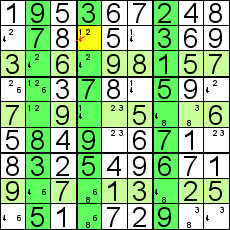
\includegraphics{images/swordfish1.png}\\
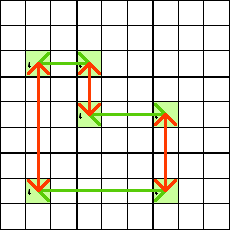
\includegraphics{images/swordfish2.png}

\end{description}

There are other rules that could be used but due to limitations these are the only implemented ones.
There are several different aspects that are interesting to note about this algorithm.
First of all the time complexity of the algorithm will be polynomial given that a solution can be found using these rules.
This is a simple consequence of the fact that each rule only take polynomial time to check and there are only polynomial many squares to fill in.
There are however no guarantee that a solution will be found and if no rule match it is impossible for the algorithm to continue.
One way around this is to combine this algorithm with the backtracking algorithm.
Other aspects that shall be studied are which rules shall be applied in which order and even if some rules are to time consuming to check compared to the extra puzzles that can be solved.
The variations of this algorithm therefore consists of different sets of rules (including guessing rules for backtracking) that are applied in different orders. 

\subsection{Boltzmann machine}
The concept of Boltzmann machines is gradually introduced by beginning with the neuron, network and finally concluding with a discussion on simulation techniques.\\

\begin{figure}[here] 
\noindent\makebox[\textwidth]{%
\begin{tabularx}{1.5\textwidth}{XX}
  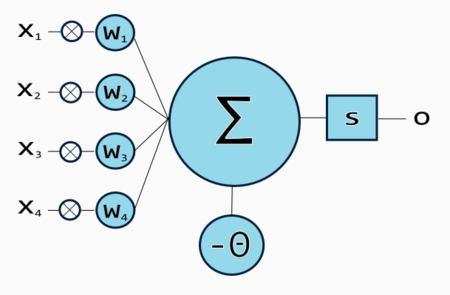
\includegraphics[width=10cm]{images/neuron.png}
\end{tabularx}}
\caption{A single neuron with showing weighted inputs from other neurons, bias threshold, and activation function.}
\label{fig:neural-Neuron}
\end{figure}
The central part of an artificial neural network (ANN) is the neuron, as pictured in \ref{fig:neural-Neuron}. .
It decides if to fire an output signal by summing upp all inputs, tresholding the value and applying an activation function producing a binary output value.
In the case of Boltzmann machines the activation function is stochastic and the probablility of a neuron being active is defined as follows:
\[
p_{i=on} = \frac{1}{1+e^{-\frac{\Delta E_{i}}{T}}}
\]
$E_i$ is the summed up energy of the whole network into neuron $i$, which is a fully connected to all other neurons.
T is a temperature constant controlling the rate of change during several evaluations with the probability $p_{i=on}$ during simulation.
$E_i$ is defined as follows \cite{boltzmann2}:
\[
\Delta E_{i} = \sum_{j} w_{ij} s_{j} - \theta
\]
where $s_j$ is a binary value set if neuron $j$ is in a active state, which occurs with probability $p_{i=on}$, and $w_{ij}$ are weights between the current node and node $j$. $\theta$ is a constant offset used to control the overall activation.

The state of every node and the associated weights describes the entire network and encondes the problem to be solved.
In the case of Sudoku there is a need to represent all 81 grid values, each having 9 possible values.
The resulting $81*9=729$ nodes are fully connected and have a binary state which is updated at every discrete timestep.
Some of these nodes will have predetermined outputs since the initial puzzle will fix certain grid values and simplify the problem.
In order to produce valid solutions it is necessary to insert weights describing known relations.
This is done by inserting negative weights, making the interconnected nodes less likely to fire at the same time, resulting in reduced probability of conflicts.
Negative weights are placed in rows, columns, 9x9 subgrids, and between nodes in the same square, since a single square should only contain a single active digit.\\

In order to produce a solution the network is simulated in discrete timesteps.
For every step, all probabilites are evaluated and states are assigned active with the given probability.
Finally the grid is checked for conflicts and no conflicts implies a valid solution, which is gathered by inspecting which nodes are in a active state.

Even though the procedure detailed above eventually will find a solution, there are enhanced techniques used in order to converge faster to a valid solution.
The temperature, $T$, can be controlled over time and is used to adjust the rate of change in the network while still allowing larger mutations to occur.
A typical scheme being used is simulated annealing (ref: http://www.sciencemag.org/content/220/4598/671.short).
By starting off with a high temperature (typically $T = 100$) and gradually decreasing the value as time progresses, it is possible to reach a global minima.
Due to practical constraints it is not possible to guarantee a solution but simulated annealing provides a good foundation which was used.\\

There are some implications of using a one-pass temperature descent which was chosen to fit puzzles as best as possible.
Typically solutions are much less likely to appear in a Boltzmann machine before the temperature has been lowered enough to a critical level.
This is due to the scaling of probabilites in the activation function.
At a big temperature all probabilites are more or less equal, even though the energy is vastly different.
With a low temperature the exponential function will produce a wider range of values, resulting in increasing probability of ending up with less conflicts.
This motivates the choice of an exponential decline in temperature over time; allowing solutions at lower temperatures to appear earlier.

\chapter{Method}
%TODO, pabergg
Since this report have several aims, this section have been divided into different parts to clearly depict what aspects have been considered regarding the different aims. 
Those sections will also describe in detail how the results was generated. 
Section 3.1 is devoted to explaining the test setup which includes hardware specifications but also an overview picture of the setup. 
Section 3.2 focuses on how and what aspects of the algorithms where analysed.
Section 3.3 explains the process of choosing test data.
The last subsection 3.4 gives an overview of the statistical analyses which was performed on the test data.
This also includes what computational limitations was present and how this effect the results. 

\section{Test setup}
%TODO HARDWARE SPECIFICATION
%Hardware: x64 x.x GHz, x GB RAM, Ubuntu x.x
%TODO: Specify compilations flag and used optimizations
The central part of the test setup was the test framework which timed and tested each algorithm on different puzzles. 
The test framework was implemented as a separate part which made it possible to guarantee correct timing and also solving correctness of the algorithms.
The algorithms was then called from the test work for each puzzle that was to be solved and the algorithm then returned when it finished.
The test framework measured the solving time and recorded it. 
Since there might be variations in processor performance multiple tests where performed on each puzzle. 
The mean value was then saved for each puzzle and algorithm.

\section{Comparison Methods}
Multiple aspects of the results was considered when analysing and comparing the algorithms. The following three subsections describes those aspects in more detail. 

\subsection{Solving}
The solving ability of an algorithm is ofcourse the most interesting aspect.
By measuring the time it takes for a sudoku to solve different puzzles one
can determine which algorithms are more effective.
Solving ability is often given in the form of a mean value, but since puzzles vary greatly in difficulty this misses the bigger picture.
An algorithm might for instance be equally good at all puzzles and one algorithm might be really good for one special kind of puzzles while performing poorly at others.
They can still have the same mean value which illustrates why that is not a good enough representation of the algorithms effectiveness.
We will therefore present histograms that shows the frequency at which it solves puzzles at a certain time intervall.
This does not only depict a more interesting view of the sudoku solvers performance, but also shows possible underlying features such as if the sudoku solver solves the puzzle with an already known distribution.
Those topics are mostly studied for each algorithm, but will also to some extent be compared between the algorithms.

\subsection{Puzzle difficulty}
One can often find difficulty ratings associated to Sudoku puzzles in puzzle books etc. 
Those are often based on the level of human solving techniques that are needed to solve the puzzle in question. \cite{difficulty} 
This study will similarly measure the puzzles difficulty, but will not rely on which level of human solving techniques that are needed, but instead on how well each algorithm performs at solving each puzzle. 
The test will primarly consist of determining if certain puzzles are inherently difficult, meaning that all algorithms rate them as hard.
During the implementation process it was discovered that the Boltzmann machine performed much worse than the other algorithms and could therefore not be tested on the same set of puzzles.
The comparison are therefore focused on the rule-based and backtracking algorithms.

\subsection{Generation and parallelization}
This is a more theoretical aspect of the comparison and no tests will be done.
It is however still possible to discuss how well the algorithms are suited for generating puzzle and how well they can be parallelisised. 
Generation of puzzles is obviously interesting because that is mainly what one want to do if constructing a puzzle collection. 
Parallelising is however not entirely obvious why it is of interest. 
Normal Sudoku puzzles can be solved in a matter of milliseconds by the best Sudoku solvers and one might therefore struggle to see the need for parallelising those solvers. 
And truly this topic is quite unrelevant for normal Sudoku puzzles but the discussion that will be held about the algorithms is however still of practical interest since one might want to solve n by n puzzles which can get extremely difficult fast when n grows. 
Since the algorithms to some extent also can be applied to other NP-complete problems, the discussion is also relevant in determining which type of algorithms might be useful in other areas. 

\section{Benchmark puzzles}
The test data consisted of multiple puzzles that was chosen beforehand.
Since the set of test puzzles can affect the outcome of this study it is appropriate to motivate the choice of puzzles.
As was discovered during the study the Boltzmann machine algorithm did not perform as well as the other algorithms and some modifications to which puzzles was used was therefore done.
The backtracking and rule-based algorithms was however both tested on a set of 49151 17-clue puzzles. 
Those was found on \cite{database} and is claimed by the author Royle to be a collection of all 17-clue puzzles that he has been able to find on the Internet. 
The reason for chosing this specific database is because the generation of the puzzles does not involve a specific algorithm but is rather a collection of puzzles found by different puzzle generating algorithms.  
The puzzles are therefore assumed to be represantative of all 17-clue puzzles. 
This assumption is the main motivating factor for chosing this set of puzzles, but there is however also other factors that makes this set of puzzles suitable. 
As recently discovered by Tugemann and Civario, no 16-clue puzzle exists which means that puzzles must contain 17 clues to have unique solutions. \cite{17clueProof}  
As discussed under section 3.2.2 difficutly rating is poorly measured by the number of clues in a puzzle, but one can however see a correlation between the number of clues and the difficulty. \cite{difficulty}
This means that the choosen set of 17-clue puzzles shall contain some of the hardest Sudoku puzzles that exists.
This is ofcourse a wanted feature since one then can see how the algorithms performs at puzzles of all difficulties.

\section{Statistical analysis}
Due to several reasons statistical analyses is required to make a rigouros statement about the results. 
This is mainly due to two reason.
Firstly the results contain a very large dataset and secondly there are some randomness in the test results which can only be dealt with by using statistical models. 
Most statistical tests give a confidence in the results to depict how surely one can be about the results of the statistical test. Naturally a higher confidence and more precise results leads to higher requirements on the statistical test. As described in section 3.4.2 some of the statistical tests have been limited by computational constraints and a lower confidence level in combination with a more inprecise result have therefore been needed for those tests.
\subsection{Statistical tests}
This section explains which statistical tests and methods are used in the study.
The first statistical method that is applied is to make sure that variance in processor performance does not affect the results considerable. 
This is done by measuring a specific algorithms solving time for a specific puzzle multiple times. 
The mean value of those times are then calculated and bootstraping are used to attain a 95\% confidence interval of 0.05 seconds. 
The reason bootstraping is used is because it does not require the stochastic variable to be a certain distribution. 
This is necessary since the distribution of the processor perfomance is unkown and also since the distribution might vary between different puzzles. \\
The meanvalues are then saved as described in section 3.1.
It is now that the real analyses of the algorithms begins. 
Even if the representation of the results does not really classify as a statistical method it is appropriate to mention that the results are displayed as histograms which means that the data are sorted and devided into bars of equal width. 
For this study this means each bar represents a fixed size solution time intervall. 
The height of the bars are proportional to the frequency data points falls into that bar's time intervall.
After the histogram are displayed one can easily compare the results between different algorithms and also consider the distribution of the solution times of individual algorithms. The usefullness of this somewhat unrigouros approach shall not negleted, but shall also use statistical methods to rigourosly prove some relations.\\
The first thing one think of looking for is probably how the different algorithms compare in solving ability. 
This means that one want to find out if one algorithm is better than other algorithms. 
Since the distribution again is unknown one has to rely on more general statistical tests. 
One of those are wilcoxons sign test. n
This makes use of the fact that the difference in solving times between two algorithms will have a mean value of 0 if there is no difference between the two algorithms. 
The tests uses the binomial theorem to see if the sign of the difference is unevenly distributed.
One can then determine if an algorithm performs better than an other algorithm with a certain confidence.
Since the distribution of the solution times are unknown it is not possible for wilcoxons sign test to give any measurement of how much better an algorithm is than another algorithm.
One might however make a histogram of the difference which leads us to the next aspect, namely difficulty rating and distribution. 
%Another approach that are also performed are to test if the test data seems to follow a certain distribution. This can be done by multiple tests.  
Difficulty rating for each algorithm can easily be calculated by making histograms of the solution times for each algorithm. 
One aim of this study have however been to determine if there is puzzles that are inherently difficult, that is regardless of solution method.
To determine if that is the case some statistical methods are required. The reader shall note that this test is only conducted on the backtracking and rulebased algorithms and the result can therefore not speak for other solution methods.
The method used is however built on the fact that independent events, say A and B, must follow the following property:
\[
P(A \cap B) = P(A) P(B)
\] 
If A is chosen to be the event that a puzzle is within algorithms 1 worst 10\% puzzles.
B is similiarly chosen to be the event that a puzzle is within the 10 \% worst puzzles for algorithm 2.
Since $P(A \cap B)$ shall den be 1 \% a statistical test can be set up to determine if the 10 \% worst puzzles are independent of algorithm. This is done by measuring the probability that the measured results appear if the null hypothesis is ascertained. If the probability is very low one can determine that the worst puzzles are not independent on the algorithms to a certain confidence level.
Similarly the easiest puzzles will be checked for independence.\\

\subsection{Computational constraints}
There is some computational constraints in the testing which have forced us to use a lower confidence level than wanted.
The problem origins from the variance in processor performance.
This was solved as discussed above by applying bootstraping to attain a approximately confidence level for the mean value to be within a certain interval.
Bootstraping is however somewhat lacking in its ability to ascertain high confidence levels for small samples compared to other methods due to the fact that it does not ascertain any special distribution.
As a result the confidence level and the allowed intervall was fitted to allow for a reasonable number of puzzles to pass with high enough confidence in a reasonable time frame.

\section{Benchmark puzzles}
This thesis relies highly on measuring how long it takes different algorithms to solve puzzles. 
To measure this, puzzles are needed and consideration shall therefore be taken to choose those puzzles wisely.
The puzzles that have been chosen to test the solving capabilities of the algorithms are a collection consisting of 49 151 puzzles which each have 17 clues (meaning 17 squares are filled in). \cite{database} Those have been collected by Gordon Royle from different sites as well as from his own database.
The reason for choosing this collection is because it is believed not to be biased towards a specific solving idea.
This is because it is a collection that comes from collecting as many of the 17-clue puzzles that have been found as possible rather than using a specific generation method.
The collection also have other benefits.
The puzzles are all qualitativly different as no pair of puzzles is within the same equivalence class.
Equivalent puzzles are defined as puzzles that could be transformed into each other using some predefined operations that doesnt change the solution.
One might for instance interchange the digits in a puzzle, but the solution would then be the transformed solution and no real change to the puzzle have therefore been done.
Some other operations includes interchanging rows, columns and stacks (three boxes in a row,column).
The downside of choosing this collection is that some algorithms may perform poorly because of the low nr of clues given and some analysis of this will therefore be carried out.
This will be done by solving the given puzzles and adding some of the numbers in the solution to the puzzle.
The reason for this approach is ones again that one does not want to rely too much on a specific generation method.

\chapter{Analysis}
%TODO, davnils/pabergg
In this section multiple results are presented together with a discussion about how the results could be interpreted. 
Section 4.1 is devoted to presenting how different algorithms perform. 
Section 4.2 explains how different puzzles can be can be correlated in terms of difficulty of solving.
%TODO: Verify the sentence above, filled in by davnils.

\section{Time distributions}
The time distributions of individual algorithms over the test set shows several things.
It is possible to observe if there is no particular difference between puzzles or if some puzzles seem to be more difficult for the algorithm to solve.

\subsection{Rule-based solver}
The rule-based solver was by far the fastest algorithm in the study and also had the lowest standard deviation. 
The result was a mean value of 0.02 seconds and a standard deviation of 0.02 seconds as well. 
The time distribution for the rule-based solver can be seen in 
figure ~\ref{fig:rule-basedDistribution}.
\begin{figure}[here] 
\noindent\makebox[\textwidth]{%
\begin{tabularx}{1.5\textwidth}{XX}
  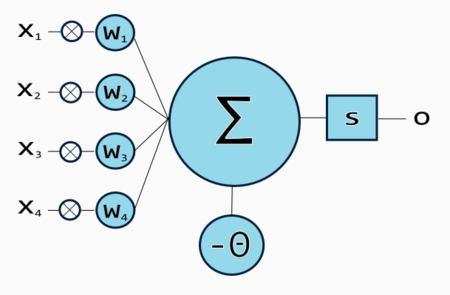
\includegraphics[width=20cm]{images/rulebaseddistribution.png}
\end{tabularx}}
\caption{A zoomed in view of the histogram showing the rule-based solvers time distribution among all 49151 puzzles. All puzzles was solved and none had an unstable measurment in running time. The confidence level for the measured solving times was 95 \% at an intervall of 0.05 seconds.}
\label{fig:rule-basedDistribution}
\end{figure}

The figure is a closed in view of the histogram showing the rule-based solvers time distribution with all 49151 puzzles. 
All puzzles were solved and all measurements were stable. The solving times was measured to be within 0.05 seconds of the recorded time with a confidence level of 95 \%. 
The maximum solution time was 1.36 seconds but as only very few measurements exceeded 0.2 seconds, those have been removed from the figure to make it clearer.
As the figure displays, the solution times increase up to a peak at about 0.17 seconds.
The solution times then drops at an approximately exponential rate.
This is believed to due to the use of backtracking.
The reason why backtracking is thought to result in this behaviour is because all search trees are believed to be equally probable and one can therefore expect to find the solution at any leaf in the search tree.
This in turn leads to the classical property of memorylessness in the exponential distribution since you can not know if

%TODO: Finish the damn sentence! /grumpy davnils

\subsection{Backtrack solver}


\subsection{Boltzmann machine solver}
%TODO: Update values and replace image with more significant results
The Boltzmann machine solver did not perform as well as others and required to be run on puzzles of difficulty 46, in order to have reasonable execution times.
Figure \ref{fig:boltzmannDistribution} shows all resulting execution times, belonging to a 95\% confidence interval of 1 second.
Only puzzles being solved within the strict 20 second limit are shown, representing TODO\% of all tested puzzles.
Given the requirement of a less strict confidence interval, due to higher variance within estimates of single puzzles, there is a higher margin of error in the results.
Inspecting the resulting distribution implies that all solved puzzles are completed within a relativily small interval, with further conclusions being limited by the margin of error. \\

A strong reason for the big representation of solutions around TODO seconds is the general layout of the Boltzmann solver.
Given that solutions are more likely to be observed at lower temperatures, as explained in the background section, it is expected to have more solutions at the end of the spectrum.
The value of TODO-TODO seconds is equivalent to a temperature of about 1\%, leading to a conclusion of this being a critical temperature for solutions to stabilze.
After this temperature interval there were no puzzles being solved within the limit of 20 seconds.

\begin{figure}[here] 
\noindent\makebox[\textwidth]{%
\begin{tabularx}{1.5\textwidth}{XX}
  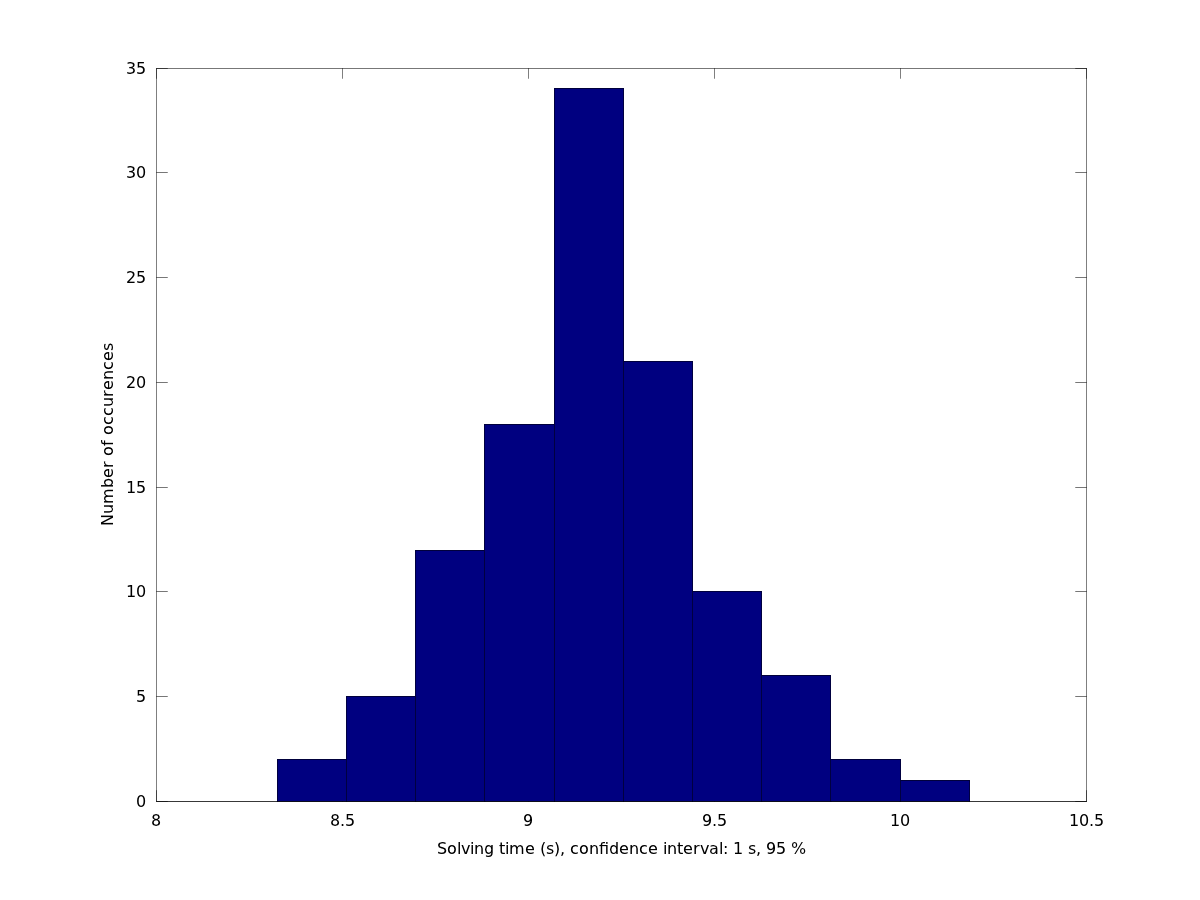
\includegraphics[width=15cm]{images/boltzmanndistribution.png}
\end{tabularx}}
\caption{Histogram showing distribution of boltzmann machine results running on TODO puzzles with 46 clues. All results belong to a 95\% confidence interval of 1 s. The image only contains puzzles being solved under the 20 second limit, which were TODO\% of all tested puzzles.}
\label{fig:boltzmannDistribution}
\end{figure}

\section{Puzzle difficulty}

\chapter{Conclusion}
%TODO: Verify all content after new data
%General structure: (1) Results (2) Conclusion (3) Future work

Three different Sudoku solvers have been studied; backtrack search, rulebased solver and Boltzmann machines.
All solvers were tested using a test framework with statistically significant results being produced.
They have shown to be dissimilar to each other in terms of performance and general behaviour.

Backtrack search and rulebased solvers are deterministic and form execution time distributions that conform to standard distributions, namely TODO and TODO.
Their excecution time was shown to have rather low variance when sampling the same puzzle repeatedly, which is believed to result from the highly deteministic behaviour.

The Boltzmann machine solver was not capable of solving harder puzzles with less clues within a reasonable timeframe.
A suitable number of clues was found to be 46 with a 20 second execution time limit, resulting in vastly worse general capabilites than the other solvers.
Due to stochastic behaviour, which is a central part of the Boltzmann solver, there was a relatively large variance when sampling the execution time of a single puzzle.
Another important aspect of the Boltzmann is the method of temperature descent, in this case selected to be simulated annealing with a single descent.
This affected the resulting distribution times in a way that makes the probability of puzzles being solved under a certain critical temperature limit high.
The temperature was found to be about TODO\% of the starting temperature, with very no puzzles being solved after this interval.

All results indicate that deterministic solvers based on a set of rules perform well and are capable of solving Sudokus with a low amount of clues.
Boltzmann machines were found to be relatively complex and requires implementation of temperature descent and adjustment of parameters.

Future work includes studying the behaviour of Boltzmann machines in relation to the final distribution of execution times.
The large variance and stochastic behaviour most likely demands a study with access to large amounts of computational power.
It is also interesting to study the influence of different temperature descents used in Boltzmann machines, with restarting being a suitable alternative to endlessly decreasing temperatures.

\chapter{References}

\begin{thebibliography}{99}

\bibitem{complexity}
Takayuki Y, Takahiro S. Complexity and Completeness of Finding Another Solution and Its Application to Puzzles. [homepage on the Internet]. No date [cited 2012 Mar 8]. Available from: The University of Tokyo, Web site: http://www-imai.is.s.u-tokyo.ac.jp/~yato/data2/SIGAL87-2.pdf

\bibitem{17clueProof}
Tugemann B, Civario G. There is no 16-Clue Sudoku: Solving the Sudoku Minimum Number of Clues Problem. [homepage on the Internet]. 2012 [cited 2012 Mar 8]. Available from: University College Dublin, Web site: http://www.math.ie/McGuire\_V1.pdf

\bibitem{enumeration}
Felgenhauer B, Jarvis F. Enumerating possible Sudoku grids. [homepage on the Internet]. 2005 [cited 2012 Mar 8]. Available from: University of Sheffield, Web site: http://www.afjarvis.staff.shef.ac.uk/sudoku/sudoku.pdf

\bibitem{techniques}
Astraware Limited. Techniques For Solving Sudoku. [homepage on the Internet]. 2008 [cited 2012 Mar 8]. Available from:, Web site: http://www.sudokuoftheday.com/pages/techniques-overview.php

\bibitem{boltzmann}
Ekeberg. Boltzmann Machines. [homepage on the Internet]. 2012 [cited 2012 Mar 8]. Available from:, Web site: http://www.csc.kth.se/utbildning/kth/kurser/DD2432/ann12/forelasningsanteckningar/07-boltzmann.pdf

\bibitem{stochastic}
Marwala T. Stochastic Optimization Approaches for Solving Sudoku. [homepage on the Internet]. 2008 [cited 2012 Mar 8]. Available from:, Web site: http://arxiv.org/abs/0805.0697

\bibitem{review}
. An Incomplete Review of Sudoku Solver Implementations. [homepage on the Internet]. 2011 [cited 2012 Mar 8]. Available from:, Web site: http://attractivechaos.wordpress.com/2011/06/19/an-incomplete-review-of-sudoku-solver-implementations/

\bibitem{discrepancySearch}
Harvey W, Ginsberg M. Limited discrepancy search. [homepage on the Internet]. No date [cited 2012 Mar 13]. Available from: University of Oregon, Web site: http://citeseerx.ist.psu.edu/viewdoc/download?doi=10.1.1.34.2426\&rep=rep1\&type=pdf

\bibitem{searchBased}
Cazenave Cazenave T. A search based Sudoku solver. [homepage on the Internet]. No date [cited 2012 Mar 13]. Available from: Université Paris, Dept. Informatique Web site: http://citeseerx.ist.psu.edu/viewdoc/download?doi=10.1.1.64.459\&rep=rep1\&type=pdf

\bibitem{culturalSwarms}
Mantere T, Koljonen J. Sudoku Solving with Cultural Swarms. AI and Machine Consciousness [homepage on the Internet]. 2008 [cited 2012 Mar 13]. Available from: University of Vaasa, Department of Electrical Engineering and Automation Web site: http://www.stes.fi/step2008/proceedings/step2008proceedings.pdf\#page=60

\bibitem{generation}
Morrow J. Generating Sudoku Puzzles as an Inverse Problem. [homepage on the Internet]. 2008 [cited 2012 Mar 13]. Available from: University of Washington, Department of Mathematics Web site: http://www.math.washington.edu/~morrow/mcm/team2306.pdf

\bibitem{database}
Royle G. Minimum Sudoku. [homepage on the Internet]. No date [cited 2012 Mar 13]. Available from: The University of Western Australia, Web site: http://www.math.washington.edu/~morrow/mcm/team2306.pdf

\bibitem{boltzmann2}
Ackley D, Hinton G. A Learning Algorithm for Boltzmann Machines. [homepage on the Internet]. 1985 [cited 2012 Mar 13]. Available from: The University of Western Australia, Web site: http://learning.cs.toronto.edu/~hinton/absps/cogscibm.pdf

\bibitem{difficulty}
%TODO Patrik: fix this reference
%http://www.sudokuwiki.org/Weekly_Sudoku.asp
blargh
\end{thebibliography}

\appendix
\addappheadtotoc
\chapter{RDF}\label{appA}

\begin{figure}[ht]
\begin{center}
And here is a figure
\caption{\small{Several statements describing the same resource.}}\label{RDF_4}
\end{center}
\end{figure}

that we refer to here: \ref{RDF_4}
\end{document}
